\chapter{Construcciones}%
\label{cha:construcciones}


\section{Imágenes inversas}%
\label{sec:imagenes_inversas}
\underline{Problema:} Hacer $f: Y \rightarrow \left( X, \mathcal{T} \right)$ continua con $\begin{cases}
    \text{topología discreta en } Y \text{ (trivialidad)}\\
    \text{topología \underline{menos fina} en } Y 
\end{cases}$. 

Es decir, buscamos crear una topología en base a $f$ de tal modo que $f$ sea siempre continua.

\underline{Solución}: 
\begin{defi}    
Llamamos \textbf{topología de la imagen inversa} a: $f^{-1} \mathcal{T} = \{f^{-1}U: U \in \mathcal{T}\}$.
\end{defi}
\begin{obs}
Con esta definición, $f$ será continua.
\end{obs}
\begin{prop}    
La topología de la imagen inversa cumple:
\begin{enumerate}
    \item Es topología. 
    \item Es mínima. 
\end{enumerate}
\end{prop}
%TODO: Acabar
\begin{demo}
    2. $f$ es continua $\Rightarrow \forall f^{-1}U$ es abierto
\end{demo}

%TODO: Fix teorema
\begin{theo}[Propiedad universal de las inmersiones]
Sean $g: \left( Z, \mathcal{T}'' \right) \rightarrow \left( Y, \mathcal{T}' \right)$ y $f: \left( Y, \mathcal{T}' \right) \rightarrow \left( Z, \mathcal{T} \right)$. Entonces:
    \[
    \mathcal{T}' = f^{-1}\mathcal{T} \Leftrightarrow  
    \]
    \begin{equation}\label{ec:prop_universal_inm}
        \left[\forall g: g \text{ cont.} \Leftrightarrow f \circ g \text{ cont.} \right]  
    \end{equation}

    \begin{figure}[H]
        \centering    
            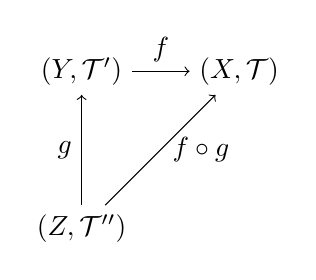
\begin{tikzpicture}[node distance=2cm, auto]
            \node(Y) {$\left( Y, \mathcal{T}' \right)$};
            \node(X) [right of=Y] {$\left( X, \mathcal{T} \right)$};
            \node(Z) [below of=Y] {$\left( Z, \mathcal{T}'' \right)$};
            \draw[->](Y) to node {$f$}(X);
            \draw[->](Z) to node [left] {$g$}(Y);
            \draw[->](Z) to node [right=0.2ex] {$f \circ g$}(X);
            \end{tikzpicture}
        \caption{\textit{Ilustración de la composición propuesta}}
        \label{prop_universal_inmersiones}
    \end{figure}
\end{theo}
\begin{demo}
\begin{itemize}
    \item $\Rightarrow)$ $\mathcal{T}' = f^{-1}\mathcal{T}: $ 
    \begin{itemize}
        \item $g$ cont. $\Rightarrow f \circ g$ cont. (Composición de continuas)
        \item $f \circ g$ cont. $\Rightarrow g$ cont. ($V \in \mathcal{T}' \Rightarrow g^{-1}V \stackrel{\mathcal{T}' = f^{-1}\mathcal{T}}{=} g^{-1} f^{-1}U = \left( f \circ g \right)^{-1} U \stackrel{f \circ g \text{ cont.}}{\in} \mathcal{T}''$)
    \end{itemize}

    \item $\Leftarrow)$ Por otro lado,
    \begin{figure}[H]
        \centering    
            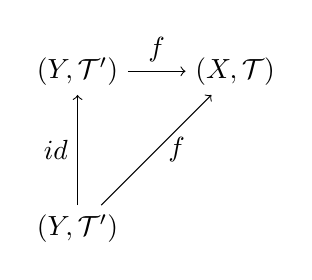
\begin{tikzpicture}[node distance=2cm, auto]
            \node(Y) {$\left( Y, \mathcal{T}' \right)$};
            \node(X) [right of=Y] {$\left( X, \mathcal{T} \right)$};
            \node(Z) [below of=Y] {$\left( Y, \mathcal{T}' \right)$};
            \draw[->](Y) to node {$f$}(X);
            \draw[->](Z) to node [left] {$id$}(Y);
            \draw[->](Z) to node [right=0.2ex] {$f$}(X);
            \end{tikzpicture}
    \end{figure}
    Como la $id$ es continua, por (\ref{prop_universal_inmersiones}), $f$ es también continua. Al ser $f^{-1}\mathcal{T}$ la menos fina, $\mathcal{T}' \supset f^{-1}\mathcal{T}$.

    Además, 
    \begin{figure}[H]
        \centering    
            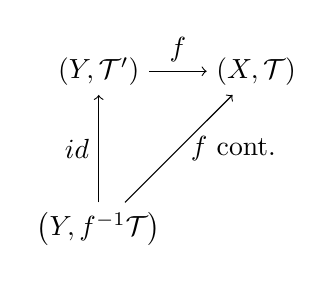
\begin{tikzpicture}[node distance=2cm, auto]
            \node(Y) {$\left( Y, \mathcal{T}' \right)$};
            \node(X) [right of=Y] {$\left( X, \mathcal{T} \right)$};
            \node(Z) [below of=Y] {$\left( Y, f^{-1}\mathcal{T} \right)$};
            \draw[->](Y) to node {$f$}(X);
            \draw[->](Z) to node [left] {$id$}(Y);
            \draw[->](Z) to node [right=0.2ex] {$f$ cont.}(X);
            \end{tikzpicture}
    \end{figure}
    Como la $f$ es continua, por (\ref{prop_universal_inmersiones}), $id$ es también continua $\Rightarrow f^{-1}\mathcal{T} \supset \mathcal{T}'$.
\end{itemize}
\end{demo}

\underline{Ejercicio}: Demostrar $\Leftarrow$) sin usar que $f^{-1}\mathcal{T}$ es la menos fina (usar que cumple la caracterización).

Caso esencial: 
\[
\boxed{f: Y \rightarrow X \text{ inyectiva}} 
\]
\begin{defi}
Una aplicación continua \textbf{inyectiva} $f: \left( Y, \mathcal{T}' \right) \rightarrow \left( X, \mathcal{T} \right)$ tal que $\mathcal{T}' = f^{-1} \mathcal{T}$ se llama \underline{inmersión}.
\end{defi}

\begin{obs}
\begin{enumerate}
    \item $\mathcal{T}' = f^{-1}\mathcal{T} \Leftrightarrow \left( Y, \mathcal{T}' \right) \xrightarrow{\text{homeo.}} \left( f\left( Y \right), \mathcal{T}|_{f\left( Y \right)} \right)$
    \begin{demo}    
    Tenemos:
    \[
    V \in f^{-1}\mathcal{T} \Leftrightarrow V = f^{-1}\underbrace{U}_{\mathcal{T}} = f^{-1}\left( \underbrace{U \cap f\left( Y \right)}_{\mathcal{T}\mid f\left( Y \right)} \right)
    \]
    \end{demo}

    \item $f: Y \rightarrow X$ $1-1$ cont. $+ \begin{cases}
        \text{ab. } \Rightarrow \text{inmersión } [\text{ab. en } X \Rightarrow \text{ab. en } f\left( Y \right)\\
        \text{cerr.} \Rightarrow \text{inmersión } [\text{cerr. en } X \Rightarrow \text{cerr. en} f\left( Y \right)] 
    \end{cases}$
    \begin{demo}
    \begin{itemize}
        \item 
        $f\left( Y \right) \stackrel{\text{ab.}}{\subset} X: V = f^{-1}U \in f^{-1}\mathcal{T} \Rightarrow fV = \overbrace{U \cap f\left( Y \right)}^{\text{inter. abiertos}} \in \mathcal{T}$.
        \item 
        $f\left( Y \right) \stackrel{\text{cerr.}}{\subset} X: C \stackrel{\text{cerr.}}{\subset}  f^{-1}\mathcal{T} \Rightarrow Y\setminus C = f^{-1} U \in f^{-1}\mathcal{T} \Rightarrow f\left( C \right) \underbrace{\left( X\setminus U \right) \cap f\left( Y \right)}_{\text{inter. cerrados}}  \stackrel{\text{cerr.}}{\subset} X$ 
    \end{itemize} 
    \end{demo}

    \item Tenemos: 
    \begin{itemize}
        \item Inmersión $ + \not$ ab. $+ \not$ cerr.
        \item Inmersión $+$ ab. $+ \not $ cerr.
        \item Inmersión $+$ ab. $+$ cerr.
    \end{itemize}
\end{enumerate}
\end{obs}

\begin{obs}
Las inmersiones permiten considerar unos espacios como subespacios de otros. Las frases ``el plano proyectivo real no es un subespacio de $\mathbb{R}^3$'', ``la esfera no es un subespacio de $\mathbb{R}^2$'', ``el plano proyectivo real es un subespacio de $\mathbb{R}^4$'' se refieren a esto: \underline{cuándo hay o no hay} una inmersión del primer espacio en el segundo, es decir, un subespacio del segundo homeomorfismo al primero. Es un problema fundamental de la topología
y de la geometría.
\end{obs}


\section{Imágenes directas}%
\label{sec:imagenes_directas}
\underline{Problema:} Hacer $f: \left( X, \mathcal{T} \right) \rightarrow Y$ continua en $\begin{cases}
    \text{top. trivial en } Y \text{(matrivialidad)}\\
    \text{top. \underline{más fina} en } Y 
\end{cases} $ 

\underline{Sol:} $f\mathcal{T} = \{V \subset Y: f^{-1}V \in \mathcal{T}\}$ top. \underline{imagen directa}.
\begin{enumerate}
    \item Es topología (inm.)
    \item Máxima [$f$ es continua $\Leftrightarrow \forall f^{-1} V$ es abierto] 
\end{enumerate}

\begin{theo}[Caracterización imágenes directas]
\begin{enumerate}
    \item
    \[
    \mathcal{T}' = f\mathcal{T} \Leftrightarrow  
    \]
    \begin{equation}
        \forall g \left[ g \text{ cont.} \Leftrightarrow g \circ f \text{ cont.} \right]
    \end{equation}

    \item Y.
    %TODO: Fix composición
    \begin{center}
        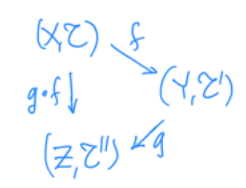
\includegraphics[scale=0.3]{images/caracterizacion_img_dir} 
    \end{center}
\end{enumerate}
\end{theo}
\begin{demo}
\begin{enumerate}
    \item $\mathcal{T}' = f^{-1}\mathcal{T}: $ 
    \begin{itemize}
        \item $g$ cont. $\Rightarrow g \circ f$ cont. (Composición de continuas)
        \item $g \circ f$ cont. $\Rightarrow g$ cont. ($W \in \mathcal{T}'' \Rightarrow f^{-1}\left( g^{-1} W \right) = \underbrace{\left( g \circ f \right)}_{\text{cont.}}^{-1} W \in \mathcal{T} \stackrel{\mathcal{T}' = f\mathcal{T}}{\Rightarrow} g^{-1}W \in \mathcal{T}'$)
    \end{itemize}

    \item Por otro lado,
    %TODO: Fix
    \begin{center}
        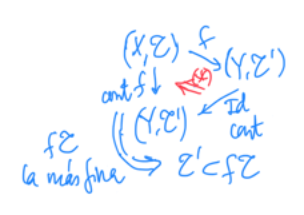
\includegraphics[scale=0.4]{images/dem_carac_img_dir_1} 
        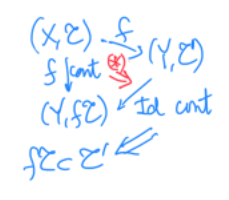
\includegraphics[scale=0.4]{images/dem_carac_img_dir_2} 
    \end{center}
\end{enumerate}
\end{demo}

\underline{Ejercicio}: Demostrar (ii) sin usar que $f\mathcal{T}$ es la más fina (usar que cumple la caracterización)

La caracterización anterior se llama \underline{propiedad universal}.

\begin{obs}
$f\left( X \right)$ es abierto y cerrado en $f\mathcal{T}: \begin{cases}
    \forall y \in Y \setminus f\left( X \right), f^{-1}y = \emptyset \in \mathcal{T} \Rightarrow \{y\} \in f\mathcal{T}\\
    f^{-1}f\left( X \right) = X \in \mathcal{T} \Rightarrow f\left( X \right) \in f\mathcal{T}
\end{cases}$
\end{obs}

Caso esencial:
\[
\boxed{f: X \rightarrow Y \text{ sobreyectiva}.} 
\]
Para entender los abiertos de una imagen directa es conveniente representarlos en el dominio. El concepto es conjuntista en realidad:

\begin{defi}
Un conjunto $A \subset X$ es \underline{saturado} (respecto de $f$) si $f^{-1}f\left( A \right) = A$.
\end{defi}
\begin{prop}
Los abiertos de $f\mathcal{T}$ son las imágenes de los abiertos saturados de $\mathcal{T}$.    
\end{prop}
\begin{demo}
\begin{enumerate}
    \item $V \in f\mathcal{T} \Rightarrow f^{-1}V \in \mathcal{T}$ y $V \stackrel{f \text{ sobre}}{=} f^{-1}fV$
    \item $U \in \mathcal{T}$, saturado $\Rightarrow f\left( U \right) = V \in f\mathcal{T}: f^{-1}V = f^{-1}f\left( U \right) \stackrel{U \text{ sat.}}{=} U \in \mathcal{T}$
\end{enumerate}
\end{demo}

\begin{obs}
Los abiertos \underline{no} saturados de $X$ pueden tener imágenes \underline{no} abiertas de $Y$. 
\end{obs}

\begin{ej}
\begin{enumerate}
    \item $f: \left[ 0, 1 \right] \rightarrow \mathbb{S}^1 = Y: t \mapsto \left( \cos 2\pi t, \sin 2\pi t \right) = \exp\left( 2 \pi i t \right)$
    %TODO: Fix image
    \begin{center}
        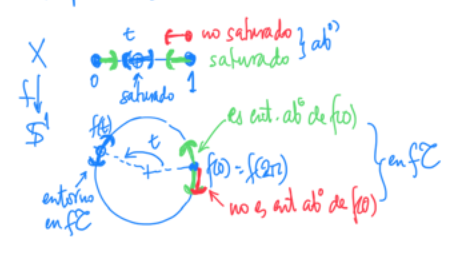
\includegraphics[scale=0.4]{images/ej_sat_1} 

        \textit{La topología imagen directa es la usual en $\mathbb{S}^1$.} 
    \end{center}

    \item Tenemos:
    \begin{align*}
        f: R = \left[ 0, 1 \right] \times \left[ 0, 1 \right] &\rightarrow C \subset \mathbb{R}^3: x^2 + y^2 = 1,\ 0 \le z \le 1\\
        \left( s, t \right) &\mapsto \left( \cos 2\pi s, \sin 2\pi s, t \right) 
    .\end{align*}

    %TODO: Fix image
    \begin{center}
        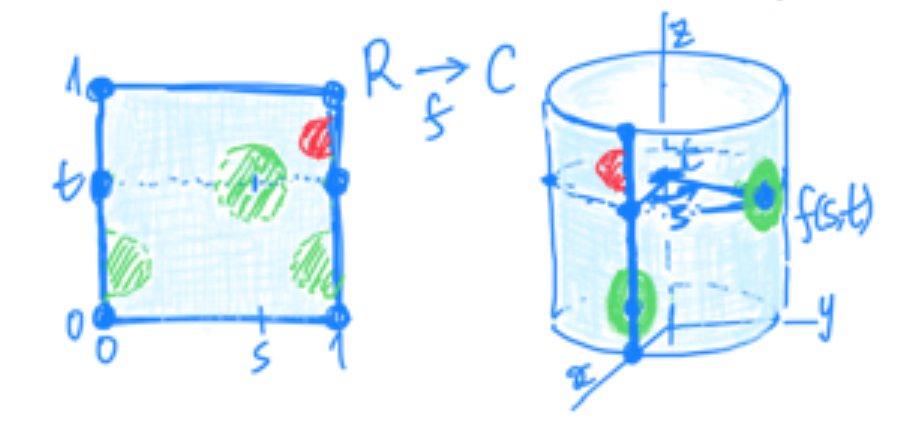
\includegraphics[scale=0.3]{images/ej_top_dir_2}

        \textit{Analizando los abiertos saturados y no saturados se concluye que la topología imagen directa es la usual en el tronco del cilindro.} 
    \end{center}
\end{enumerate}
\end{ej}

\begin{defi}
Una aplicación continua sobre $f: \left( X, \mathcal{T} \right) \rightarrow \left( Y, \mathcal{T}' \right)$ tal que $\mathcal{T}' = f\mathcal{T}$ se llama \underline{identificación} (se suelen omitir las topologías)
\end{defi}

\begin{obs}
\begin{enumerate}
    \item Identificación: $V \stackrel{\text{ab}}{\subset} Y \Leftrightarrow f^{-1}V \stackrel{\text{ab}}{\subset} X$

    Continua: $V \stackrel{\text{ab}}{\subset } Y \Rightarrow f^{-1}V \stackrel{\text{ab}}{\subset} X$

    \item Sea $f: X \rightarrow Y$ sobre. continua. Si además es:
    \begin{itemize}
        \item Abierta $\Rightarrow f$ es identificación [por (1)]
        \item Cerrada $\Rightarrow f$ es identificación [$f^{-1}V \stackrel{\text{ab}}{\subset} X \stackrel{\text{+ cerr.}}{\Rightarrow} f\left( \underbrace{X \setminus f^{-1}\left( V \right)}_{= Y\setminus V} \right) \stackrel{\text{cerr.}}{\subset} Y \Rightarrow V \stackrel{\text{ab}}{\subset} Y$
    \end{itemize}
\end{enumerate}
\end{obs}

\begin{defi}[Cociente]
Dentro de las identificaciones tenemos un caso particular: $\left( X, \mathcal{T} \right) \stackrel{p}{\rightarrow} Y = \underbrace{X / \sim}_{p \mathcal{T} = \text{top. cociente}}$. Cociente respecto de una relación de equivalencia en $X$. 
\end{defi}
%TODO: Fix imagen
\begin{center}
    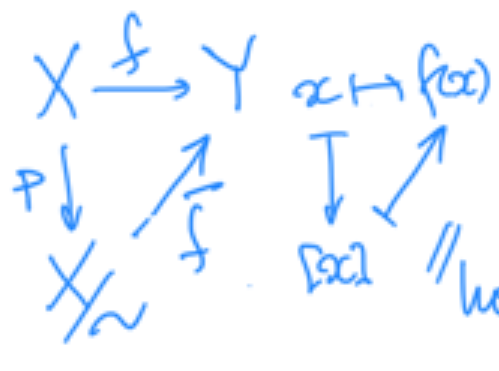
\includegraphics[scale=0.2]{images/def_cociente} 
\end{center}
Tenemos que $x_1 \sim x_2 \stackrel{\text{def}}{\Leftrightarrow} f\left( x_1 \right) = f\left( x_2 \right)$. Homeoforma de $p\mathcal{T}$ sobre $f\mathcal{T} \Leftrightarrow f$ identificación tal que:
\[
\begin{cases}
    \overline{f} \text{ es biyección}\\
    p^{-1}V = f^{-1}\overline{f} V \text{ y } f^{-1}W = p^{-1} \overline{f}^{-1}W
\end{cases} 
\]

\begin{pg}
    Los cocientes son cómodos para definir espacios, las identificaciones son mejores para estudiar las propiedades que tenemos. Conviene pues tener triángulos como el anterior. Se puede contemplar $Y$ como un modelo del cociente.
\end{pg}

%TODO: Fix imágenes
\begin{ej}[Anteriores]
La circunferencia y el cilindro como cocientes:
\begin{center}
    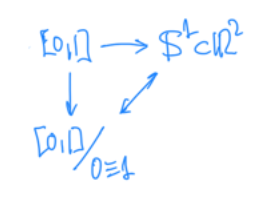
\includegraphics[scale=0.4]{images/ej_cociente_1} 
    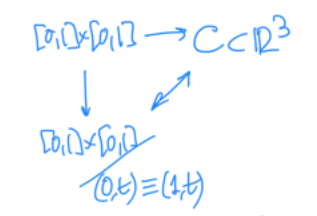
\includegraphics[scale=0.4]{images/ej_cociente_2}
\end{center}

Para representar cocientes se utilizan dibujos que indican las identificaciones en los espacios de partida:
%TODO: Fix
\begin{center}
    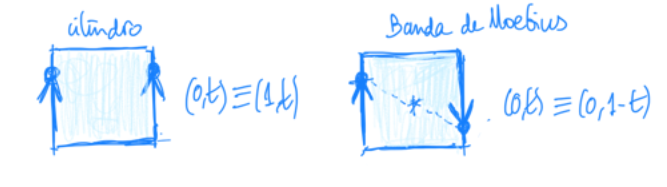
\includegraphics[scale=0.3]{images/ej_cociente_3} 
\end{center}
\end{ej}


\section{Productos (finitos)}%
\label{sec:productos_finitos_}
\underline{Problema:} Hacer $X_1 \times \ldots \times X_r = Y \xrightarrow{p_i} \left( X_i, \mathcal{T}_i \right), 1 \le i \le r$ continuas con 
\[
\begin{cases}
    \text{top. discreta en } Y \text{ matrivialidad}\\
    \text{top. \underline{menos fina} en} Y
\end{cases} 
\]
\underline{Solución:} $p_i$ cont. $\Rightarrow p_i^{-1} \underbrace{U_i}_{\mathcal{T}_i} = \underbrace{X_1 \times \ldots \times U_i \times \ldots \times X_r}_{\text{deben ser abiertos}}  \Rightarrow \bigcap_{i} p_i^{-1}U_i = \underbrace{U_1 \times \ldots \times U_r}_{\text{abiertos}}$ pero \underline{no} son topología $\Rightarrow$
\[
\mathcal{B} = \{U_1 \times \ldots \times U_r: U_i \in \mathcal{T}_i \} \text{ es la \underline{base} de la \underline{topología producto}: } \boxed{\prod_{i} \mathcal{T}_i} 
\]
\begin{ej}
La $\mathcal{T}_u$ en $\mathbb{R}^n$ ese el producto de la usual en cada factor $\mathbb{R}$ de $\mathbb{R}^n$. La base de la definición de topología producto está formada por las ``bolas cuadradas''.
\end{ej}

%TODO: Fix teorema
\begin{theo}[Caracterización topología producto]
\begin{enumerate}
    \item
    \[
    \mathcal{T}' = \prod_{i} \mathcal{T} \Leftrightarrow  
    \]
    \begin{equation}
        \forall g \left[ g \text{ cont.} \Leftrightarrow \forall g_i \text{ cont.} \right]
    \end{equation}

    \item Y.
    %TODO: Fix composición
    \begin{center}
        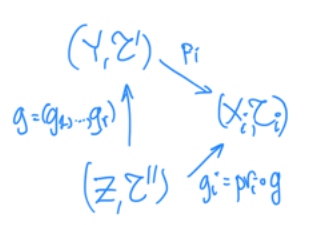
\includegraphics[scale=0.3]{images/caracterizacion_top_prod} 
    \end{center}
\end{enumerate}
\end{theo}
\begin{demo}
\begin{enumerate}
    \item $\mathcal{T}' = \prod_{i} \mathcal{T}: $ 
    \begin{itemize}
        \item $g$ cont. $\Rightarrow g_i$ cont. (Composición de continuas)
        \item $g_i$ cont. $\Rightarrow g^{-1}\left( U_1 \times \ldots \times U_r \right) = \underbrace{g_1^{-1}\left( U_1 \right)}_{\mathcal{T}''} \cap \ldots \cap \underbrace{g_r^{-1}\left( U_i \right)}_{\mathcal{T}''} \in \mathcal{T}''$ (intersección finita de abiertos) 
    \end{itemize}

    \item Por otro lado,
    %TODO: Fix
    \begin{center}
        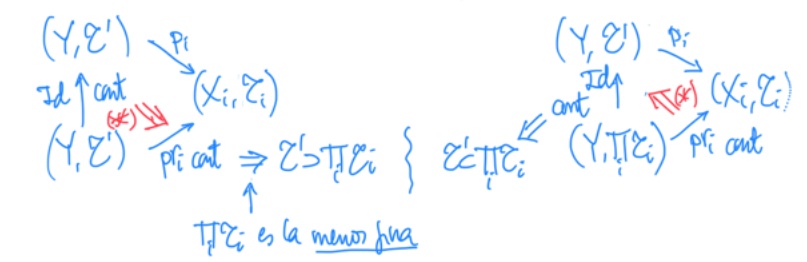
\includegraphics[scale=0.4]{images/dem_carac_top_prod} 
    \end{center}
\end{enumerate}
\end{demo}

\begin{ej}
Demostrar (ii) sin usar que $\prod_{i} \mathcal{T}_i$ es la menos fina (usar que cumple la caracterización)
\end{ej}

La anterior caracterización se llama \underline{propiedad universal}.

\begin{prop}
\begin{enumerate}
    \item $p_i: Y \rightarrow X_i$ es abierta. [$p_i\left( U_1 \times \ldots \times U_r \right) = U_i$]
    \item $X_j \xrightarrow{\alpha_j} Y: x_j \mapsto \left( a_1, \ldots, x_j, \ldots, a_r \right)$ es inmersión ($a_i \in X_i$ fijados).
    \[
    \left[\begin{cases}
        \alpha_j\left( X_j \right) = \{a_1\} \times \ldots \times X_j \times \ldots \times \{a_r\} \\
        \alpha_j\left( U_j \right) = \{a_1\} \times \ldots \times U_j \times \ldots \times \{a_r\} = \alpha\left( X_j \right) \cap \left( X_1 \times \ldots \times U_j \times \ldots \times X_r \right) 
    \end{cases}\right]     
    \]
\end{enumerate}
\end{prop}

\begin{pg}
En una topología producto ``todo se genera en productos''.
\begin{ej}
\begin{itemize}
    \item Bases de entornos: $\mathcal{V}^a = \mathcal{V}^{a_1} \times \ldots \times \mathcal{V}^{a_r} \stackrel{mut??}{=} \{V_1 \times \ldots \times V_r: V_i \in \mathcal{V}^{a_i}\} \left( a \in Y \right)$.
    \item Base de abiertos: $\mathcal{B} = \mathcal{B}_1 \times \ldots \times \mathcal{B}_r = \{B_1 \times \ldots \times B_r: B_i \in \mathcal{B}_i\}$ (esto repite la construcción de $\prod_{i} \mathcal{T}_i$)
\end{itemize}
\end{ej}
\end{pg}


\section{Sumas (finitas)}%
\label{sec:sumas_finitas_}
\underline{Problema:} Hacer $\left( X_i, \mathcal{T}_i \right) \xrightarrow{e_i} Y = X_1 + \ldots X_r = \left( X_1 \times \{1\} \right) \cup \ldots \cup \left( X_r \times \{r\} \right), 1 \le i \le r: x_i \mapsto \left( x_i, i \right)$ continuas, ,con 
\[
\begin{cases}
    \text{top. trivial en } Y \text{ matrivialidad}\\
    \text{top. \underline{más fina} en} Y
\end{cases} 
\]
\underline{Solución:} $\underbrace{U_i}_{\mathcal{T}_i} \in e_i^{-1}\left( U_i \times \{i\} \right) \Rightarrow \mathcal{B} = \{U_1 \times \{1\}, \ldots, U_r \times \{r\}: U_1 \in \mathcal{T}_1, U_r \in \mathcal{T}_r\}$ es base de una topología en $Y$, la topología \underline{suma}: $\mathcal{T}_1 + \ldots + \mathcal{T}_r$.

\begin{prop}
$\forall i, e_i: \left( X_i, \mathcal{T}_i \right) \rightarrow \left( X_i\times \{i\}, \mathcal{T}|_{X_i \times \{i\}} \right)$ es inmersión abierta y cerrada.
\end{prop}
\begin{demo}
\begin{itemize}
    \item Inmersión abierta: $e_i\left( U_i \right) = U_i \times \{i\} \in \mathcal{T}$
    \item Cerrada: $Y\setminus e_i\left( X_i \right) = Y \setminus X_i \times \{i\} = \bigcup_{j \neq i} X_j \times \{j\} \in \mathcal{T}$
\end{itemize}
\end{demo}

%TODO: Fix teorema
\begin{theo}[Caracterización topología suma]
\begin{enumerate}
    \item
    \[
    \mathcal{T}' = \mathcal{T}_1 + \ldots + \mathcal{T}_r \Leftrightarrow  
    \]
    \begin{equation}
        \forall g \left[ g \text{ cont.} \Leftrightarrow \forall g_i \text{ cont.} \right] \text{(Propiedad universal)} 
    \end{equation}

    \item Y.
    %TODO: Fix composición
    \begin{center}
        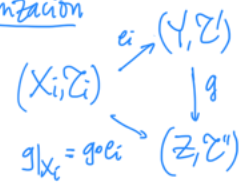
\includegraphics[scale=0.3]{images/caracterizacion_top_sum} 
    \end{center}
\end{enumerate}
\end{theo}
%TODO: Tal vez hacerlo bien?
\begin{demo}
    Análoga a las anteriores construcciones.
\end{demo}

\begin{pg}
Localmente $Y = X_1 + \ldots + X_r$ es como sea cada $X_i$. Por ejemplo, las bases de entornos de $Y$ son las de los sumandos. Globalmente, se trata cada sumando separadamente. Por ejemplo, las bases de abiertos de los sumandos se unen para dar una base de abiertos de $Y$. Olvidando el tecnicismo $X_i \times \{i\} \equiv X_i$:
\begin{center}
   $Y$ es unión disjunta de los sumandos\\
   Los sumando son subespacios abiertos y cerrados de $Y$
\end{center}
Es un formalismo para hacer cómodamente otras construcciones. Por ejemplo, ``pegar dos discos por sus bordes'' sería:
\begin{gather*}
    \text{disco} D \subset \mathbb{R}^2: x^2 + y^2 \le 1, \text{ borde } \partial D = \mathbb{S}^1: x^2 + y^2 = 1\\
    %TODO: Fix cociente
    D_1 + D_2 / \sim\quad \overbrace{\left( p, 1 \right)}^{\partial D} \sim \left( p, 2 \right) 
.\end{gather*}
%TODO Fix
\begin{center}    
    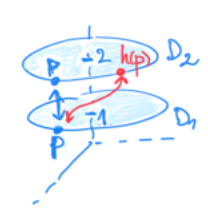
\includegraphics[scale=0.3]{images/pg_top_sum} 
\end{center}
y más elaborado $h: \partial D \stackrel{\text{homeo.}}{\approx} \partial D$ con $\overbrace{p}^{\in \partial D} \sim h\left( p \right)$.

Finalmente, hay otros conceptos de ``suma'' más significativos que veremos en algún ejemplo.
\end{pg}


\section{Espacios proyectivos reales}%
\label{sec:espacios_proyectivos_reales}
Como vimos en geometría lineal tenemos que: 
\[
\mathbb{R}P^n = \mathbb{P}^{n} = \mathbb{R}^{nH}\setminus \{0\} / \underbrace{\sim }_{\text{Prop.}} \Rightarrow \mathbb{P}^{n} = \{\text{rectas vectoriales de } \mathbb{R}^{n+1}\}     
\]
Que en coordenadas es:
\begin{align*}
    \pi: \mathbb{R}^{nH} \setminus \{0\} &\rightarrow \mathbb{P}^{n}\\
    \left( x_0, \ldots, x_n \right) &\mapsto \left( x_0 : \ldots : x_n \right) 
.\end{align*}
Las ecuaciones serán de la forma: $h\in \mathbb{R}\left[ x_0, \ldots, x_n \right]$ homogénea $\Rightarrow \begin{cases}
    h\left( x \right) = 0\\
    h\left( x \right) \neq 0
\end{cases}$ está bien definido en $\mathbb{P}^{n}$.
\[
\begin{rcases}
    %TODO: Fix lista
   \text{· Variedades proyectivas lineales}\\  
   \text{· Variedades proyectivas}\\
   \text{· Variedades proyectivas algebraicas}  
\end{rcases} \text{ecuaciones homogéneas de grado:} 
\begin{cases}
    1\\
    2\\
    \text{arbitrario} 
\end{cases} 
\]
\underline{Cartas afines:} 
\begin{gather*}
    \underbrace{H \subset \mathbb{P}^{n}}_{\text{hiperplano proyectivo}} \rightarrow \underbrace{\hat{H} \subset \mathbb{R}^{n + 1}}_{\text{hiperplano lineal} } : \underbrace{h = 0}_{\text{forma lineal}}, H = \hat{H} \setminus \{0\} / \sim  \\
    \pi|: \underbrace{\{h = 1\} \subset \mathbb{R}^{n + 1} \setminus \{0\}}_{\text{hiperplano afín}} \rightarrow \underbrace{\mathbb{P}^{n} \setminus H}_{\{h \neq 0\}} = 0 \text{ es biyección.}    
.\end{gather*}
Terminología: $H$ es \underline{hiperplano del infinito} de la \underline{carta afín} $U$.

Topología en $U$: La imagen directa de la usual en $\{h = 1\} \subset \mathbb{R}^{n + 1} \Rightarrow \pi|: \{h = 1\} \rightarrow U$ \underline{homeomorfismo}. 

%TODO: Fix subrayado
\underline{Topología en }$\mathbb{P}^{n}$: 
\begin{itemize}
    \item \underline{Cociente} de la usual vía $\mathbb{R}^{n+1}\setminus \{0\} \xrightarrow{\pi} \mathbb{P}^{n}: \left( x_0, \ldots, x_n \right) \mapsto \left( x_0 : \ldots : x_n \right)$
    \item ``\underline{Suma}'' de las definidas en las cartas afines:
    \[
        W \text{ abierto si } W \cap U \text{ es abierto } \forall U \text{ carta afín. [Es top. en } \mathbb{P}^{n}] 
    \]
\end{itemize}
Estas dos topologías coinciden.
\begin{demo}
\begin{enumerate}
    \item $U$ es abierto en la top. cociente. [$\pi^{-1} U = \{h \neq 0\}$ abierto usual]
    \item La topología cociente en $U$ coincide con la topología de carta afín:
    %TODO: Fix diagrama
    \begin{center}
        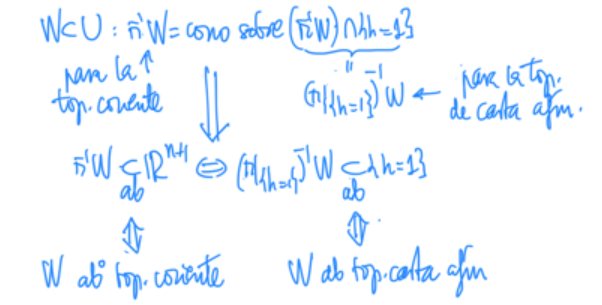
\includegraphics[scale=0.3]{images/eq_top_proyectivo} 
    \end{center}
    \item[1. + 2.] $\Rightarrow $ La top. cociente está generada por las topologías de las cartas afines, que forman un recubrimiento abierto de $\mathbb{P}^{n}$.
\end{enumerate}
\end{demo}

\begin{obs}
De lo anterior deducimos:
\begin{enumerate}
    \item $U_1, U_2$ dos cartas afines $\Rightarrow U_1 \cap U_2$ abiertos.
    \[
    \left[ \text{Cartas afines: } U_i = \{h_1 \neq 0\} \begin{cases}
        \pi|: \{h_1 = 1\} \rightarrow U_1 \text{homeo.}\\
        \left( \pi_1 \right)^{-1}\left( U_1 \cap U_2 \right) = \{h_1 = 1, h_2 \neq 0\} \stackrel{\text{ab.}}{\subset} \{h_1 = 1\}  
    \end{cases} \right] 
    \]
    \item Las topologías de $U_1$ y $U_2$ coinciden en $U_1 \cap U_2$.

    [De nuevo conviene entenderlo con cartas:
    %TODO: Fix
    \begin{center}
        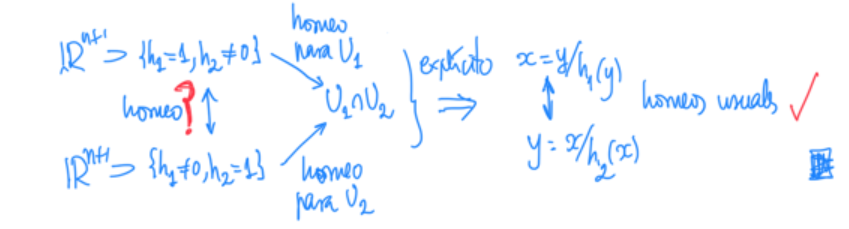
\includegraphics[scale=0.3]{images/obs_cartas_afines} ]
    \end{center}
\end{enumerate}
\end{obs}

%TODO: Esto es posible que se pueda agrupar mejor (hasta Möbius)
\underline{Atlas afín canónico}: No se suelen utilizar todas las cartas afines: $n + 1$ distintas ya cubren $\mathbb{P}^{n}$. Típicamente $\mathbb{P}^{n} = U_0 \cup \ldots \cup U_n$ con:
\[
U_i = \{x_i \neq 0\} \leftrightarrow \{\underbrace{x_i = 1}_{\equiv \mathbb{R}^n}\}: \left( x_0 : \ldots : x_i : \ldots : x_n \right) \mapsto \left( \frac{x_0}{x_i}, \ldots, \overbrace{1}^{\mathbb{R}^n \rightarrow}, \ldots, \frac{x_n}{x_i} \right), 0 \le i \le n
\]

\underline{Cociente antipodal}: Toda recta de $\mathbb{R}^{n + 1}$ corta a $\mathbb{S}^{n}: x_0^2 + \ldots + x_n^2 = 1$ en dos puntos \underline{antipodales}, así que denotamos un ``sub'' cociente, que es también identificación.
%TODO: Fix imagen
\begin{center}
    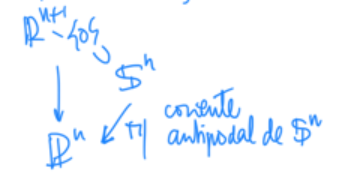
\includegraphics[scale=0.3]{images/cociente_antipodal} 

    [Como antes tenemos conos: $\pi^{-1}W = $ cono sobre $\underbrace{\mathbb{S}^n \cap \pi^{-1}W}_{= \left( \pi / \mathbb{S}^n \right)^{-1} W}$]
\end{center}

Las cartas afines tienen una representación muy conveniente:
%TODO: Fix imagen
\begin{center}
    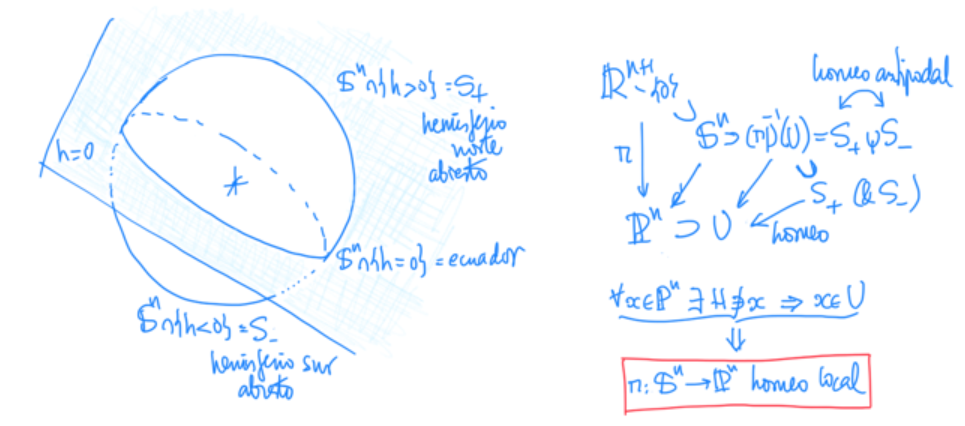
\includegraphics[scale=0.3]{images/repr_carta_afin} 
\end{center}

\underline{Cociente de un disco}:
\[
E = \{h = 0, x_0^2 + \cdots + x_n^2 = 1\} = \partial \begin{cases}
    \overline{S}_+ = \mathbb{S}^n \cap \{h \ge 0\} \text{ hemisferio cerrado.} \\
    D^n = \{h = 0, x_0^2 + \cdots + x_n^2 \le 1\} \text{ disco.} 
\end{cases} 
\]
%TODO: Fix imagen
\begin{center}
    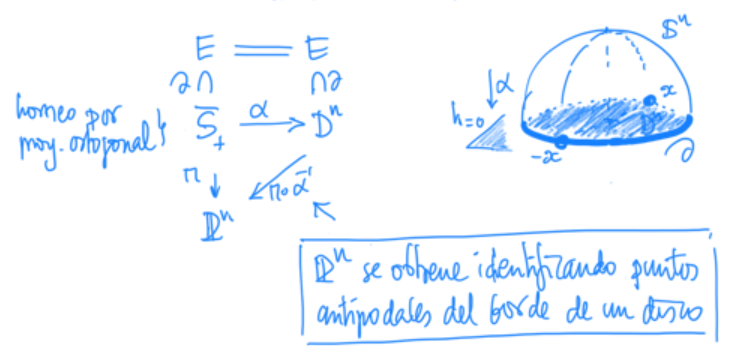
\includegraphics[scale=0.3]{images/cociente_disco} 
\end{center}

\begin{ej}
$\mathbb{P}^{2} \setminus D^2 = $ banda de Möbius.
%TODO: Fix imagen
\begin{center}
    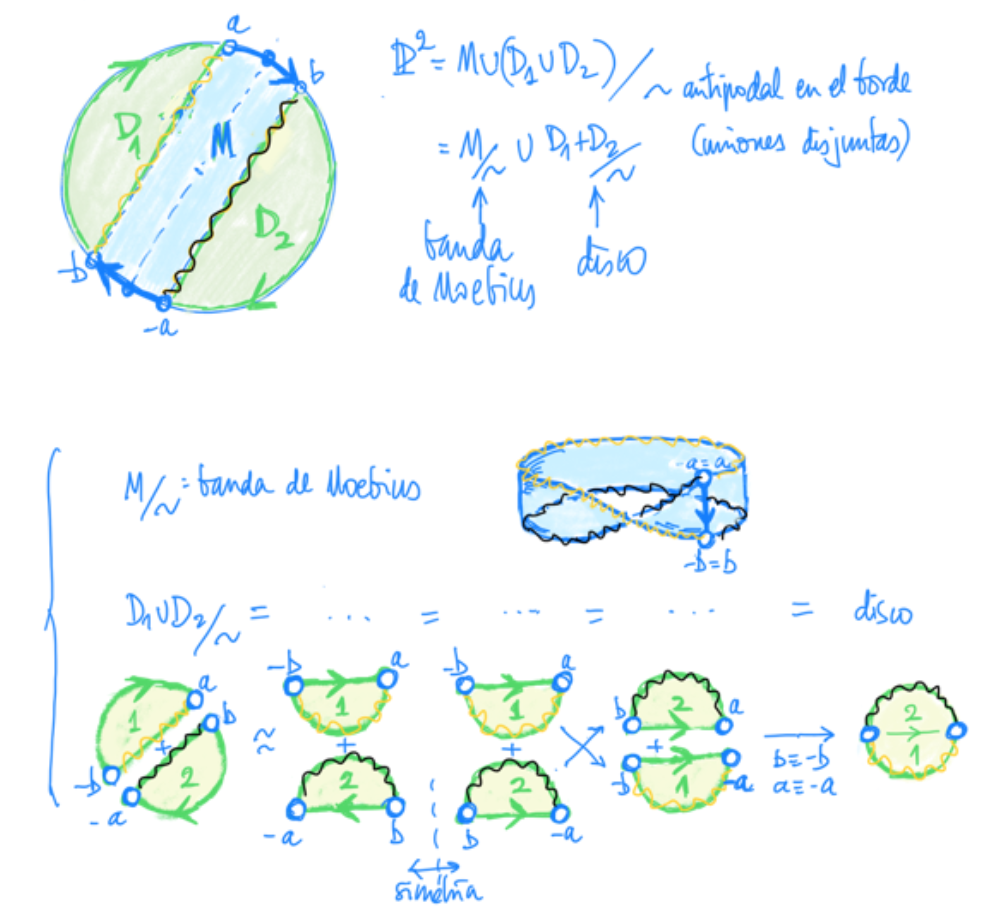
\includegraphics[scale=0.3]{images/banda_moebius} 
\end{center}
\end{ej}

